\testCom
{%Номер задачи
	3.128
}
{%Условие
	условие
}
{%Дано
	дано
}
{%Найти
	найти
}
{%Решение
	%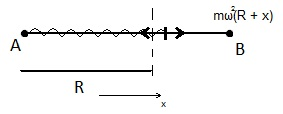
\includegraphics[height=30mm]{3_33.jpg}\\
	Дифференциальное уравнение, описывающее физический процесс:\\
	\[ \der{q}{t}{2} = \frac{R}{L} \der{q}{t}{} + \frac{1}{LC} q = 0\]
	В момент максимума тока: $ \der{q}{t}{2} = 0$\\
	нужно найти - $\frac{CL ( \der{q}{t}{2})}{q^2}$\\
	$\frac{R^2}{\cancel{L^2}} = \frac{1}{\cancel{L^2} C^2} q^2$\\
	$\frac{CL}{q^2} \cdot ( \der{q}{t}{})^2 = \frac{L}{CR^2}$\\
}

